%%
%% Copyright 2007, 2008, 2009 Elsevier Ltd
%%
%% This file is part of the 'Elsarticle Bundle'.
%% ---------------------------------------------
%%
%% It may be distributed under the conditions of the LaTeX Project Public
%% License, either version 1.2 of this license or (at your option) any
%% later version.  The latest version of this license is in
%%    http://www.latex-project.org/lppl.txt
%% and version 1.2 or later is part of all distributions of LaTeX
%% version 1999/12/01 or later.
%%
%% The list of all files belonging to the 'Elsarticle Bundle' is
%% given in the file `manifest.txt'.
%%

%% Template article for Elsevier's document class `elsarticle'
%% with numbered style bibliographic references
%% SP 2008/03/01
%%
%%
%%
%% $Id: elsarticle-template-num.tex 4 2009-10-24 08:22:58Z rishi $
%%
%%
\documentclass[final,3p]{elsarticle}

%% Use the option review to obtain double line spacing
%% \documentclass[preprint,review,12pt]{elsarticle}

%% Use the options 1p,twocolumn; 3p; 3p,twocolumn; 5p; or 5p,twocolumn
%% for a journal layout:
%% \documentclass[final,1p,times]{elsarticle}
%% \documentclass[final,1p,times,twocolumn]{elsarticle}
%% \documentclass[final,3p,times]{elsarticle}
%% \documentclass[final,3p,times,twocolumn]{elsarticle}
%% \documentclass[final,5p,times]{elsarticle}
%% \documentclass[final,5p,times,twocolumn]{elsarticle}

\usepackage{hyperref}
\usepackage[capitalize]{cleveref}

%% if you use PostScript figures in your article
%% use the graphics package for simple commands
%% \usepackage{graphics}
%% or use the graphicx package for more complicated commands
\usepackage{graphicx}
%% or use the epsfig package if you prefer to use the old commands
%% \usepackage{epsfig}

\usepackage{caption,subcaption}
\usepackage{float}

%% The amssymb package provides various useful mathematical symbols
\usepackage{amssymb}
%% The amsthm package provides extended theorem environments
%% \usepackage{amsthm}

%% The lineno packages adds line numbers. Start line numbering with
%% \begin{linenumbers}, end it with \end{linenumbers}. Or switch it on
%% for the whole article with \linenumbers after \end{frontmatter}.
%% \usepackage{lineno}
\usepackage{amsmath}
\usepackage{xfrac}

% Modify citation style.
\usepackage[numbers]{natbib}

% Packages for custom table views.
% The multirow package provides merged row cells, while booktabs allows customizing the lines.
\usepackage{multirow, booktabs}
% These packages allow colors in table.
\usepackage{color, colortbl}

% Chinese support
\usepackage{xeCJK}
\setCJKmainfont{Lantinghei TC}

%% natbib.sty is loaded by default. However, natbib options can be
%% provided with \biboptions{...} command. Following options are
%% valid:

%%   round  -  round parentheses are used (default)
%%   square -  square brackets are used   [option]
%%   curly  -  curly braces are used      {option}
%%   angle  -  angle brackets are used    <option>
%%   semicolon  -  multiple citations separated by semi-colon
%%   colon  - same as semicolon, an earlier confusion
%%   comma  -  separated by comma
%%   numbers-  selects numerical citations
%%   super  -  numerical citations as superscripts
%%   sort   -  sorts multiple citations according to order in ref. list
%%   sort&compress   -  like sort, but also compresses numerical citations
%%   compress - compresses without sorting
%%
%% \biboptions{comma,round}

% \biboptions{}

\journal{LS1012 General Biology Lab, 106-1}

% adjust the footer
\makeatletter
\def\ps@pprintTitle{%
 \let\@oddhead\@empty%
 \let\@evenhead\@oddhead
 \def\@oddfoot{\centerline{\thepage}}%
 \let\@evenfoot\@oddfoot}
\makeatother

% custom color
\definecolor{Gray}{gray}{0.9}

\begin{document}

\begin{frontmatter}

\title{作業二 Video Captioning}

\author{劉彥廷~B03902036}

\end{frontmatter}

%%
%% Start line numbering here if you want
%%
% \linenumbers

\section{模型敘述}
	\begin{figure}[H]
		\centering
		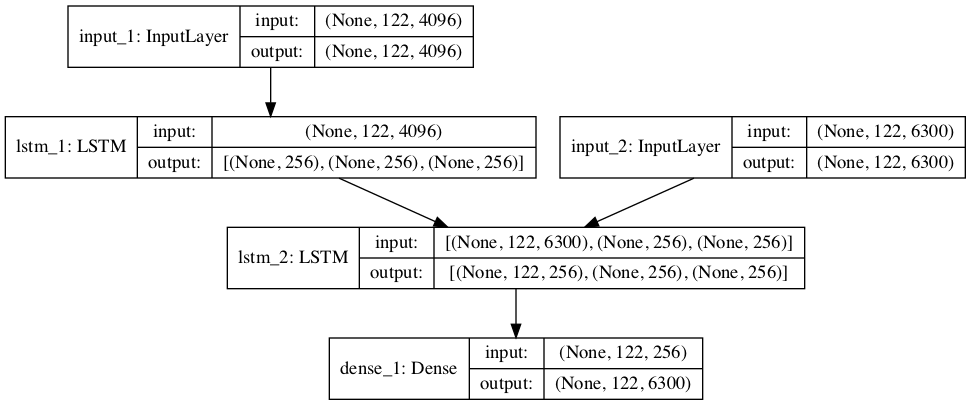
\includegraphics[width=0.7\textwidth]{images/model}
		\caption{繳交的模型} \label{fig:model}
	\end{figure}
	
	模型參照了 \cite{keras10} 的介紹,一層 RNN 作為編碼器(encoder),並且在處理完輸入的序列後回傳內部的狀態,提供給下一層作為解碼器(decoder)的 RNN。
	身為解碼器的 RNN 會讀入兩種輸入,一種為來自編碼器的狀態,另外一種則為做為標準答案的 one-hot 文字向量。
	
	在本次的實作當中,one-hot 的字典檔維度為 6300 字。而測試的資料總共有 1450 筆獨立的影片,每個影片個字會有的註解(caption)總共創造出 24232 筆不重複的訓練資料組。
	
	\subsection{Attention}
	本次並沒有實作出 attention 的結果,但如果要實作出來,只需要在 lstm\_1(請參見程式)添加額外的 Dense 層,並且反饋給來自 lstm\_2 的 Dense 層即可。
			
\section{優化方式}
	本次作業使用了 teacher force(請參閱前述的文章)的方式來減少訓練的複雜度。
		
\section{結果}
	本次作業並沒有實作完畢 attention model,加上花了太久的時間在處理 dataset,沒有足夠的時間訓練出合適的結果。
		
%% References
%%
%% Following citation commands can be used in the body text:
%% Usage of \cite is as follows:
%%   \cite{key}         ==>>  [#]
%%   \cite[chap. 2]{key} ==>> [#, chap. 2]
%%

%% References with bibTeX database:
\bibliographystyle{apa}
% \bibliographystyle{elsarticle-num} 
% \bibliographystyle{elsarticle-harv}
% \bibliographystyle{elsarticle-num-names}
% \bibliographystyle{model1a-num-names}
% \bibliographystyle{model1b-num-names}
% \bibliographystyle{model1c-num-names}
% \bibliographystyle{model1-num-names}
% \bibliographystyle{model2-names}
% \bibliographystyle{model3a-num-names}
% \bibliographystyle{model3-num-names}
% \bibliographystyle{model4-names}
% \bibliographystyle{model5-names}
% \bibliographystyle{model6-num-names}

\section{參考文獻}
\bibliography{reference}

%% The Appendices part is started with the command \appendix;
%% appendix sections are then done as normal sections
% Have the appendices start with a new page.
%\newpage
%\appendix
	
\end{document}
